\documentclass [10 pt, xcolor=pdftex,x11names,table]{beamer} 
\usepackage{pgf, pgfpages}
\usepackage[latin1]{inputenc} 
\usepackage[english]{babel}
%\usepackage{beamerhighlight}
\usepackage{colortbl}
\usepackage{color}
\usepackage{pdfpages}
\usepackage[absolute,overlay]{textpos}
\usepackage{url}
\usepackage{graphicx}
\usepackage{mathtools,amssymb,mathrsfs,amsthm,amsmath,graphicx,float}
\usepackage[linesnumbered,ruled,vlined]{algorithm2e}
\graphicspath{{../figures/}}
\newcommand{\Gv}{G_{\mathit{\sigma_v}}}
\newcommand{\Gx}{G_{\mathit{\sigma_x}}}
\DeclareMathOperator\erf{erf}

\mode<presentation>
{
    \usetheme{Madrid}
    \usecolortheme{beaver}
    \usefonttheme{professionalfonts} 
    \setbeamertemplate{itemize item}{$\blacktriangleright$}
    \setbeamertemplate{itemize subitem}{$\blacktriangleright$}
    \setbeamertemplate{enumerate items}{$\blacksquare$}
    \setbeamercolor{enumerate item}{fg=red!80!black}
    \setbeamercolor{itemize item}{fg=black!80!white}
    \setbeamercolor{itemize subitem}{fg=black!80!white}

}

\usepackage{hyperref}
\title{\sc \bf Smoothed Local Histogram Filters}
\subtitle{Sparsity and Compressed Sensing}
\author{\bf Maha ELBAYAD}
\institute[MVA|ECP]{\large{Ecole CentraleSupelec | ENS Cachan (M2 MVA)} }
\date{\today}

\begin{document}

\begin{frame}
    \titlepage
\end{frame}
\begin{frame}[label=Overview]
    \frametitle{Overview}
    \begin{enumerate}
    \item Motivation
    \item Smooth Local Histograms
    \item Morphological filters
    \item Mode filters
    \item Applications
    \end{enumerate}   
\end{frame}

\section{Motivation}    
\begin{frame}[label=Motivation]
    \frametitle{Motivation}
\begin{itemize}
\item An image histogram specifies the intensities distribution within the whole image: \textbf{It does not contain spatial information.}

\item Local histograms summarize the tonal distribution within an image neighborhood.

\item Many applications in computer vision make use of the smooth local histograms (SLH).

\item \textcolor{red}{Caveat:} Very expensive computation over large neighborhoods.\\$\mathcal O(n^2\log n)$: binned histogram of neighborhood size $(n\times n)$
\end{itemize}
\end{frame}

\section{Smooth local histograms}
\begin{frame}[label=SLH1]
    \frametitle{Definition}
    \textbf{Density estimation:}
    The SLH can be seen as a kernel density estimator:
    \[\hat f_p(s) = \sum_i K(I_{q_i}-s)W(p-q_i)\]
    Where (values space parameters):
    \setbeamertemplate{itemize item}{-}
    \begin{itemize}
    \item $K$ is the smoothing kernel, generally a gaussian kernel of wifth $\sigma_v$ denoted by $\Gv$.
    \item $I_{q_i}$ the intensity of the pixel $q_i$ in $p$'s neighborhood/
    \item $s$ the shift
    \item we sample the shift values $(s_i)_{1\leq i\leq m}$ at a frequency larger than the Nyquist frequency.
    \end{itemize}

    \begin{center}\framebox{$f_p(s) = \Gv(I_p - s) \otimes W$}\end{center}

    \centerline{\textcolor{black!70}{The kernel shouldn't introduce additional extrema}}
\end{frame}

\begin{frame}[label=SLH2]
    \frametitle{Definition}
    \textbf{Density estimation:}
    The SLH can be seen as a kernel density estimator:
    \begin{center}\framebox{$f_p(s) = \Gv(I_p - s) \otimes W$}\end{center}
    Where (spatial space parameters):
    \setbeamertemplate{itemize item}{-}
    \begin{itemize}
    \item $W$ is a weighting function positive, has unit sum and ideally with valued diminishing with distance.
    \item Generally we consider $W$ a gaussian kernel window with width = $\sigma_x$ 
    \end{itemize}
        \begin{center}\includegraphics[width=6cm]{kernels}\end{center}

    
\end{frame}

\begin{frame}
    \frametitle{Integration and derivation}
    \textbf{Derivative}
\[\forall i\{1,..,m\},\: D_i(p)=\frac{1}{\sigma_v^2}(I_p-s_i)K(I_p-s_i)\otimes W\]
We interpolate the signal $(D_i(p))_i$ to approximate the value of $D(I_p)$ and locate:
\begin{itemize}
\item The modes (local maxima : negative going zero crossings of $D_p$).
\item The antimodes (local minima: positive going zero crossings of $D_p$) 
\end{itemize}
\begin{center}\includegraphics[width=7cm]{modes}\end{center}
\end{frame}


\begin{frame}
    \frametitle{Integration and derivation}
    \textbf{Integral}
    \[R_i(p) = \phi(I_p-s_i)\otimes W\]
    Where for the Gaussian kernel $\Gv$:
    \[\phi(z) = \sigma_v \sqrt{\frac{\pi}{2}} \left(1 + \erf\left(\frac{z}{\sigma_v\sqrt{2}}\right)\right)\]
    Whenever we need to evaluate $R(I_p)$ or $D(I_p)$ we linearly interpolate between two consecutive shifts such that $I_p\in[s_i,s_{i+1}]$.\\
    \textcolor{red}{The sampling frequency should be large enough to ensure sufficient approximations.}
\end{frame}

\section{Morphological filters}

\begin{frame}[label=Morpho]
    \frametitle{Morphological filters}
    The morphological filter of order $\beta$ outputs the $\beta-$percentile of the intensities within the neighborhood. i.e.
    \[\mathbb P(I\leq x) = \beta\]
    \begin{center}
    \includegraphics[width=8cm]{int}
    \end{center}
\end{frame}
\begin{frame}[label=Morpho]
    \frametitle{Morphological filters : Particular cases}
    \textbf{Median: }$\mathbf{\beta = 50\%}$\\
    \textbf{Erosion: }$\mathbf{\beta = 5\%}$\\
    {\footnotesize The default erosion filter consider the minimum intensity in the neighborhood in case $W$ is the unit area, to integrate the spatial variation we set $\beta$ for the erosion at $5\%$.}

    \textbf{Dilation: }$\mathbf{\beta = 95\%}$\\
     {\footnotesize The default erosion filter consider the maximum intensity (we move $\beta$ from 100\% to 95\%).}

    \textbf{Closing: } Erosion followed by dilation

    \textbf{Opening: } Dilation followed by erosion.
    \begin{center}
    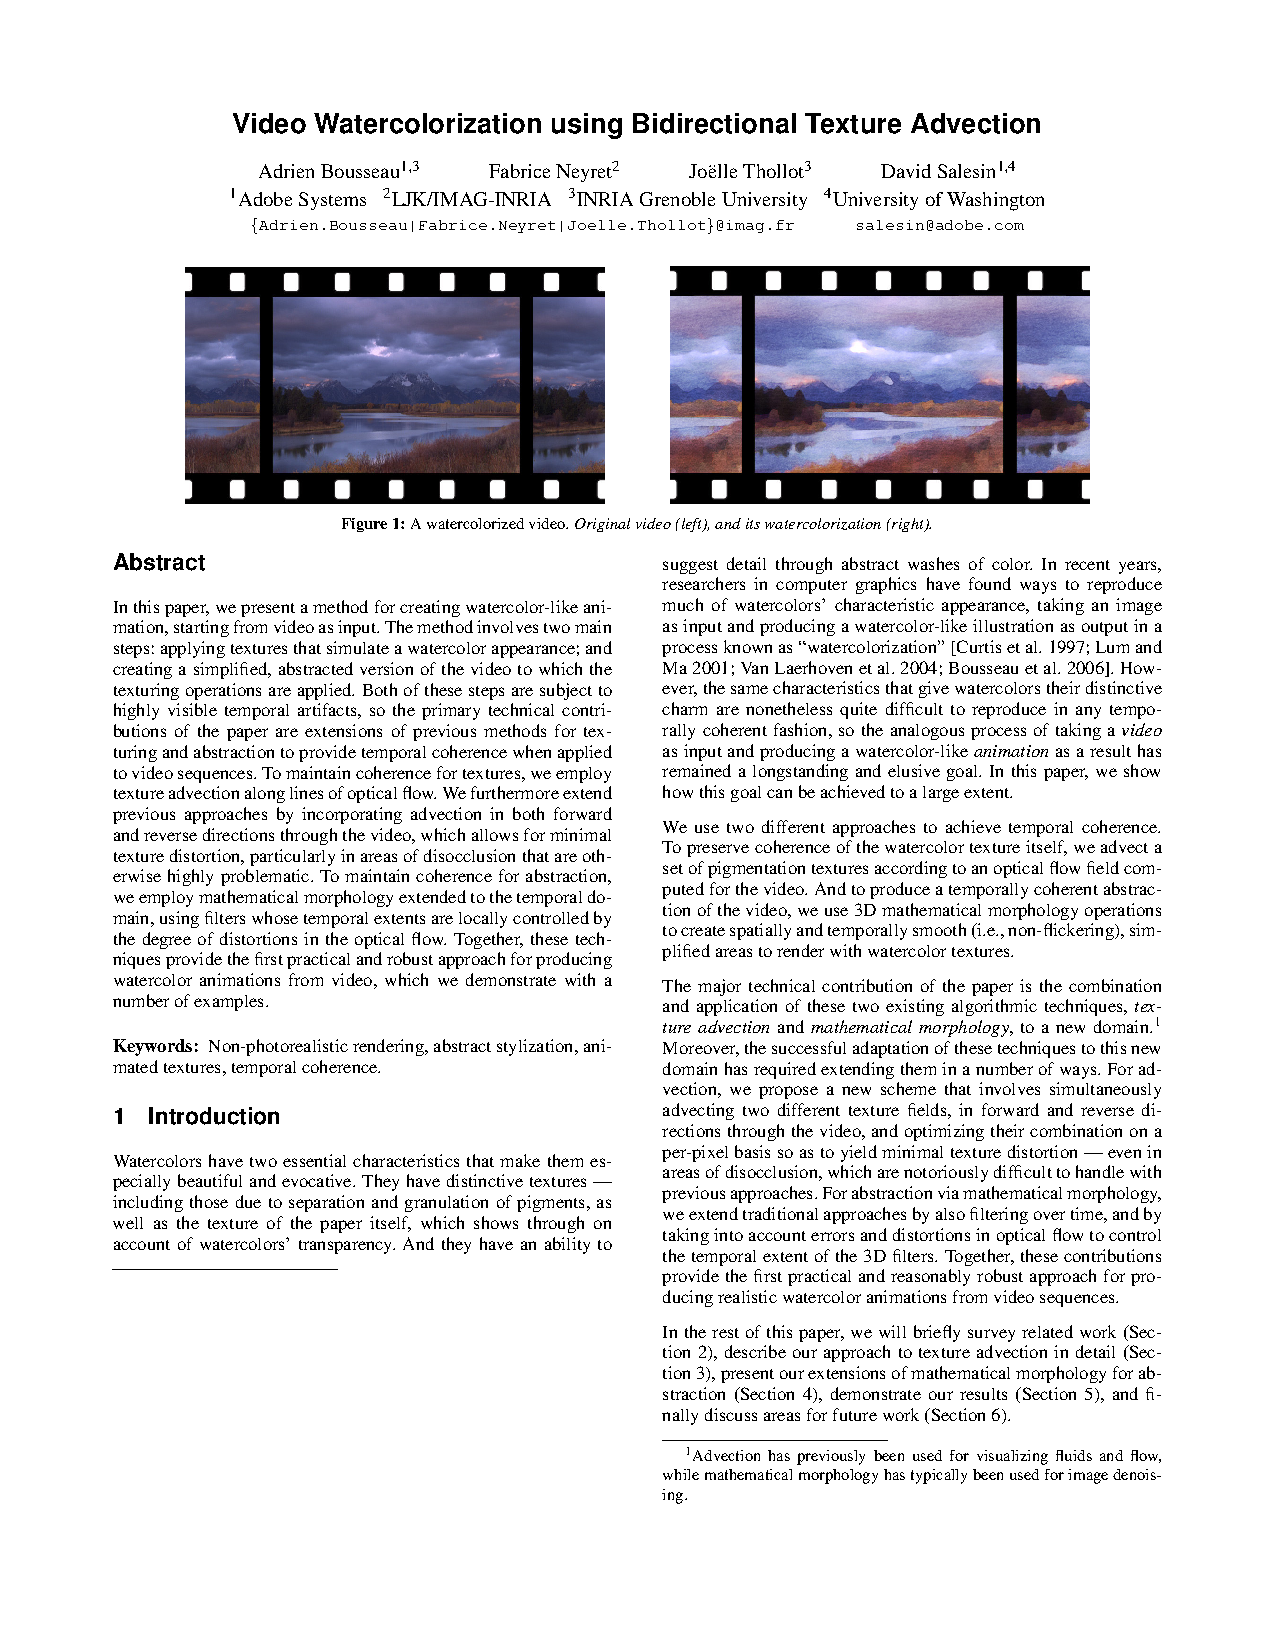
\includegraphics[width=5.5cm]{bousseau}
    \end{center}
\end{frame}

\section{Mode filters}

\begin{frame}
    \frametitle{Mode filters}
     \textbf{Closest mode:}\\
     It's the mode one would reach by steepest ascent in the smoothed local histogram. \\
   
     \begin{itemize}
     \item Estimate $D(I_p)$
     \item if $D(I_p)\geq 0$, select the first mode greater than $I_p$.
     \begin{itemize} \item otherwise, select the largest mode smaller than $I_p$.\end{itemize}
     \end{itemize}
    \textcolor{red}{Relies heavily on the input value.}

    \textbf{Dominant mode:}\\
     Choose the mode with the largest population:\\
     population $\approx$ area between the two antimodes surrounding the considered mode
    \begin{center}
    \includegraphics[width=5cm]{dominant_hist}
    \end{center}
\end{frame}

\begin{frame}
    \begin{center}
    \includegraphics[width=10cm]{tractor}
    \end{center}
\end{frame}

\section{Applications}

\begin{frame}
\frametitle{Detail enhancement}
     \textbf{Selective Diffusion:}\\
     \begin{itemize}
     \item Decompose an image into a base layer and an additional detail layer.
     \item Find the base layer with an edge-preserving filter
     \item Diffuse the base layer with gaussian blurring.
     \end{itemize}
\begin{center}
    \includegraphics[width=8cm]{dog}
    \end{center}
\end{frame}

\begin{frame}
\frametitle{Detail enhancement}
     \textbf{Iterative selective Diffusion:}\\
     \begin{itemize}
     \item Reiterate the selective diffusion over the detail layer.
     \end{itemize}
    \begin{center}\framebox{$I = \left(\sum\limits_{i=1}^n\mathcal B_i\right) + \mathcal D_n$}\end{center}

\begin{center}
    \includegraphics[width=8cm]{moon}
    \end{center}
\end{frame}

\begin{frame}[allowframebreaks]
\frametitle{References}

\bibliographystyle{acmsiggraph}
\nocite{*}
\bibliography{template}

\end{frame}
\end{document}





